\section{Atom-field interactions}
%%
\subsection{Introduction}
The electric-dipole Hamiltonian is:
\begin{align}
    \highlight{
    H_{int}=-\hbd\cdot\hbE(\br_A),\quad 
    \begin{array}{l}
        \bd=\text{Atomic dipole moment}\\
        \bE=\text{E-field at the position of the atom}
    \end{array}}.
\end{align}
\begin{itemize}[itemsep=0pt,topsep=0pt]
    \item Interaction between a classical dipole and classical E-field: models of atom polarizability.
    \item Interaction between a quantized atom structure (two-level) and classical EM-field: Raby cycle, quantum 
    logic states, 3-level systems.
    \item Interaction between a single atom and quantuzed EM-field (free space): spontaneous emission, Lamb shift,
    caivty WED, Purcell effect, etc.
    \item Multiple atoms and quantized EM field: dipole-dipole interactcions, collective spontaneous emission.
    \item Single atom, classical field, quantized motion: atom cooling and trapping, atom interferometry.
    \item Single atom (polarizable particle), quantized field, etc.
\end{itemize}
%%
\subsection{Atom-matter interaction}
At the most fundamental level light-matter interaction reduces to the interaction between EM fields and 
single atoms, which are composed of charges.

Let us consider the atom to be a distribution of charges $\{q_n,m_n\}$ located at $\br_n$ relative to the 
atomic center of mmass $\br_A$.
\begin{figure}[htbp]
    \centering
    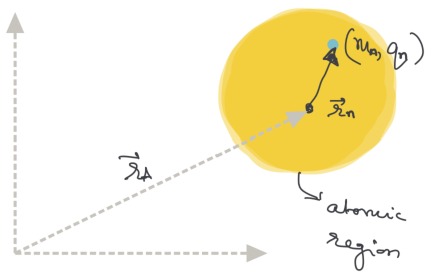
\includegraphics[width=.3\columnwidth]{PartOne/ChapterFour/figures/atomdistribution.png}
    \caption{Atom distribution and distribution of charges.}
\end{figure}

The Lorentz force on a charge is:
\begin{align}
    \bF(\br)=q\bE(\br)+q\bv\times\bB(\br).
\end{align}
The corresponding electric and magnetic potentials are:
\begin{align}
    V_e&=\text{Electric potential}=-\int\;d\bs\cdot\sum_nq_n\delta(\bs-\br_n)\bE(\br_A+\bs),\\
    V_m&=\text{Magnetic potential}=-\int\;d\bs\cdot\sum_nq_n\delta(\bs-\br_n)\bv_n\times\bB(\br_A+\bs).
\end{align}
We note that the variation of the EM-fields over the size of th atom is small. 

\begin{definition}[Review of Bohr model]
    \begin{align*}
        \text{Centrifugal force=electrostatic force ($z=1$)}\qquad\frac{m_ev_n^2}{r_n}=\frac{1}{4\pi\varepsilon_0}\frac{e^2}{r_n^2}\longrightarrow m_ev_n^2r_n=\frac{e^2}{4\pi\varepsilon_0}.
    \end{align*}
    \begin{align*}
        \text{Quantization of angular momentum}\qquad m_ev_nr_n=n\hbar
    \end{align*}
    Dividing the above equations:
    \begin{align*}
        v_n=\frac{e^2}{4\pi\varepsilon_0n\hbar}.
    \end{align*}
    Assuming $n=1$:
    \begin{align*}
        v=\frac{e^2}{4\pi\varepsilon_0\hbar},
    \end{align*}
    Substituting in the first expression:
    \begin{align*}
        r=\frac{\hbar}{m_ev}=\frac{4\pi\varepsilon_0\hbar^2}{m_ee^2},
    \end{align*}
    Transition wavelength:
    \begin{align*}
        \lambda=\frac{2\pi\hbar c}{E}=\frac{4\pi\hbar c}{m_ev^2},\quad E=\frac{1}{2}m_ev^2.
    \end{align*}
    \begin{align*}
        \frac{r}{\lambda}\sim\frac{\hbar}{m_ev}\frac{m_ev^2}{2\pi\hbar c}=\frac{v}{2\pi c}=\frac{e^2}{4\pi\varepsilon_0\hbar c}=\alpha.
    \end{align*}
\end{definition}





We note that the ratio of atomic radius to transition wavelength $r/\lambda$ ad the ratio of speed of $e^-$ in 
orbit to speed of light $v/c$ are both of the order of $\alpha$, the fine-structure constant.

From this we conclude that the variation of the EM-fields over the size of the atom is small.
Let us compare the size of the magnetic to electric potential:
\begin{align}
    \left|\frac{V_m}{V_e}\right|\sim\frac{|\bv||\bB|}{|\bE|}\stackrel{\text{Ampere's law}}{\sim}\frac{|\bv|}{c}\sim\frac{e^2}{4\pi\varepsilon_0\hbar c}\equiv\alpha\approx\frac{1}{137}.
\end{align}
Magnetic interactions between atoms and EM fields are waker by a factor of $\alpha$ compared to electric interactions.

Let us look at the electric potential:
\begin{align*}
    V_e&=-\int\;d\bs\cdot\sum_nq_n\delta(\bs-\br_n)\bE(\br_A+\bs)\\
    &=-\sum_nq_n\underbrace{\Phi(\br_A+\br_n)}_{\text{scalar potential}}\quad(\text{Sifting property of delta})\\
    &=-\sum_nq_n\left[\Phi(\br_A)+\br_n\cdot\nabla\Phi(\br_A)+\text{higher order terms}\right]\\
    V_e&=-\underbrace{\sum_nq_n}_{=0(\text{neutral atom})}\Phi(\br_A)-\underbrace{\sum_nq_n\br_n}_{=\bd (\text{dipole moment})}\cdot\bE(\br_A)+\text{multipolar terms}.
\end{align*}
Thus, the atom-field interaction under the electric-dipole approximation is given by:
\begin{align}
    \highlight{V_e=-\bd\cdot\bE(\br_A)\xrightarrow{\text{Quantization}}\hH_{int}=-\hbd\cdot\hbE(\br_A)}.
\end{align}
